% =============================================================================
% Capítulo 5 · Resultados (avance) y discusión
% Redactado el 7-nov-2026 con autorización explícita de Roberto para presentarlo como avance en
% MMC102 (regla 7: no se publica en el sitio). Fuentes: data/results/final/ (16 series, niveles),
% notebooks 05, 06, 06c, 07b, 07c y 09a, R/ciclo_financiero_final.Rmd y los dictámenes de la
% iteración 3b. Toda cifra entra por macro de cifras.tex; las que faltan se definen en
% cifras_stub.tex como \pendiente con su archivo de origen. Las lecturas cualitativas (signos,
% composición de grupos, etiquetas) se toman de los mismos archivos.
% =============================================================================
\chapter{Resultados (avance) y discusión}
\label{cap:resultados}

Este capítulo presenta el avance de resultados con las \nSeries{} series vigentes, sin
transformar, de \fechaInicioNiveles{} a \fechaFinDatos{}. Sigue el orden de la cadena del
\cref{cap:metodologia}: los datos y su adecuación (\cref{sec:res-datos}); el PCA estático y su
dimensión (\cref{sec:res-pca}); la tendencia y el nulo de tendencias (\cref{sec:res-tendencia});
la parte dinámica, con el EPCA, los umbrales por ventana, el criterio de ancho de ventana y las
transiciones (\cref{sec:res-dinamica}); la HFC (\cref{sec:res-hfc}); la datación de regímenes
(\cref{sec:res-datacion}); su contraste con los episodios de referencia
(\cref{sec:res-validacion}), y el estado del complemento de aprendizaje profundo
(\cref{sec:res-dl}). La \cref{sec:res-discusion} discute qué sostienen y qué no los resultados
frente a las hipótesis de trabajo.

Tres advertencias enmarcan la lectura. Primero, es un \textbf{avance}: la interpretación es
prudente y queda sujeta a la discusión con el asesor; en particular, la Parte~C de la decisión D2
(qué aspecto del ciclo mide cada vía y cómo se combinan) sigue pendiente
(\cref{sec:pend-parte-c}), y los resultados se presentan sin adelantarla. Segundo, conforme al
principio «datos primero», cada resultado se describe antes de interpretarlo, y se contrasta con
la referencia que corresponde (un nulo, una sensibilidad o un episodio externo) antes de
atribuirle un significado económico. Tercero, toda cifra se genera desde los archivos de
resultados; las que aún no tienen macro se muestran como pendientes, con el nombre de la macro y
el archivo del que saldrá.

% -----------------------------------------------------------------------------
\section{Datos y adecuación muestral}
\label{sec:res-datos}

La matriz de datos tiene $n=\nMesesNiveles$ meses y $p=\nSeries$ series, sin valores faltantes y
con calendario continuo (\cref{sup:datos}); la \cref{fig:res-correlaciones} muestra su matriz de
correlaciones. Se distinguen a simple vista dos bloques de correlación alta: el de los agregados
de crédito y liquidez, que se mueven junto con los precios, la actividad y las reservas, y el de
las tasas de interés de corto plazo. El EMBIG y el índice bursátil se relacionan con ambos bloques
de forma más débil, y entre sí con signo negativo.

\begin{figure}[htbp]
\centering
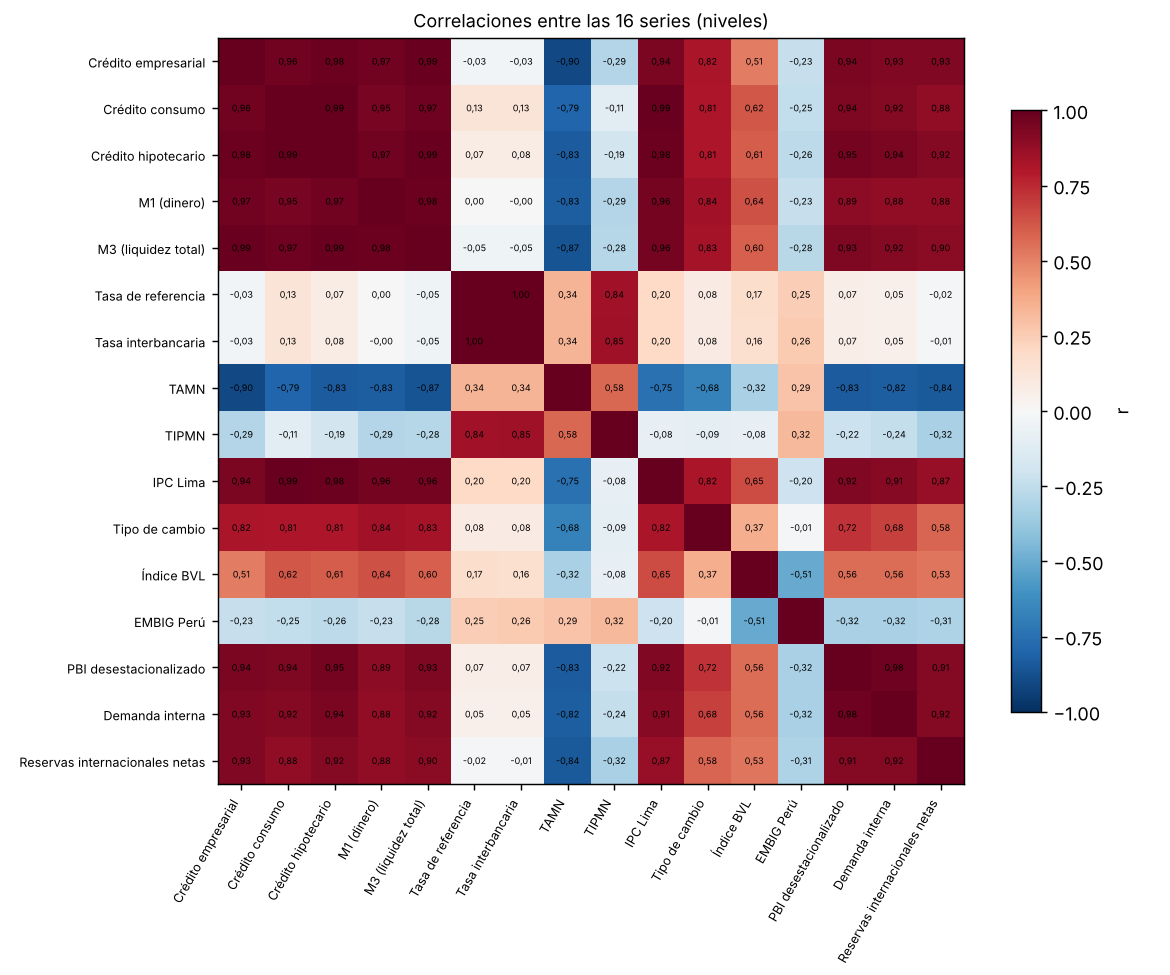
\includegraphics[width=0.85\textwidth]{final/05_correlaciones.png}
\caption{Matriz de correlaciones de las series sin transformar}
\label{fig:res-correlaciones}
\par\smallskip
{\footnotesize Fuente: \texttt{reports/figures/final/05\_correlaciones.png} (notebook 05).}
\end{figure}

La medida de adecuación global es $\KMO=\kmoGlobalNiveles$ (\cref{def:kmo}): las correlaciones se
explican, en su mayor parte, por lo que cada serie comparte con las demás, y no por pares aislados.
Las medidas individuales más bajas son las de la tasa de referencia (\kmoTasaReferencia{}), la tasa
interbancaria (\kmoTasaInterbancaria{}) y el EMBIG (\kmoEmbig{}). En las dos tasas, el resultado es
el esperable si son casi colineales, como sugieren sus cargas casi idénticas en el segundo eje
(\cref{sec:res-pca}): una correlación parcial alta entre ambas reduce su medida individual. La prueba
de esfericidad de Bartlett (\cref{def:bartlett}) da $\chi^2_{\mathrm B}=\chiBartlettNiveles$ con
\glBartlett{} grados de libertad, pero esa cifra no tiene la distribución de referencia, porque los
meses no son independientes (\cref{obs:bartlett-series}). Si se reemplaza $n$ por la mediana del
tamaño muestral efectivo entre pares de series, que es apenas \nEfMedianaNiveles{}, el estadístico
baja a \chiBartlettNefNiveles{} y su p-valor a \pBartlettNefNiveles{}. El número de condición de
$\mR$ es \numCondicionNiveles{}: hay combinaciones de series casi colineales.

\emph{Lectura.} Hay estructura común que resumir, pero su evidencia formal es mucho más débil de
lo que sugiere la prueba ingenua: con series tan persistentes, \nMesesNiveles{} meses equivalen,
para una correlación, a unas pocas observaciones independientes. Por eso las medidas de
adecuación se leen como descripciones de $\mR$, no como pruebas (\cref{obs:bartlett-series}).

% -----------------------------------------------------------------------------
\section{PCA estático y número de dimensiones}
\label{sec:res-pca}

\paragraph{Inercia y retención.} Los cuatro primeros ejes retienen \inerciaPCUnoNiveles\,\%,
\inerciaPCDosNiveles\,\%, \inerciaPCTresNiveles\,\% y \inerciaPCCuatroNiveles\,\% de la inercia; los
tres primeros, \inerciaAcumTresNiveles\,\% (\cref{fig:res-sedimentacion}). Los criterios de
retención no coinciden (\cref{sec:retencion}): el análisis paralelo de Horn retiene
\hornNiveles{} ejes, la vara quebrada \varaQuebradaNiveles{} y el criterio de Kaiser
\kaiserNiveles{}. El desacuerdo está en el tercer eje: su valor propio, \lambdaTresNiveles{},
supera el umbral de Kaiser, pero no el de Horn, \hornUmbralTresNiveles{}. La decisión D9 fijó
$d=3$ antes de conocer estas cifras, de modo que el tercer eje se interpreta, con la salvedad de
que dos de los tres criterios no lo retienen; $d=2$ y $d=4$ se informan como sensibilidad.

\begin{figure}[htbp]
\centering
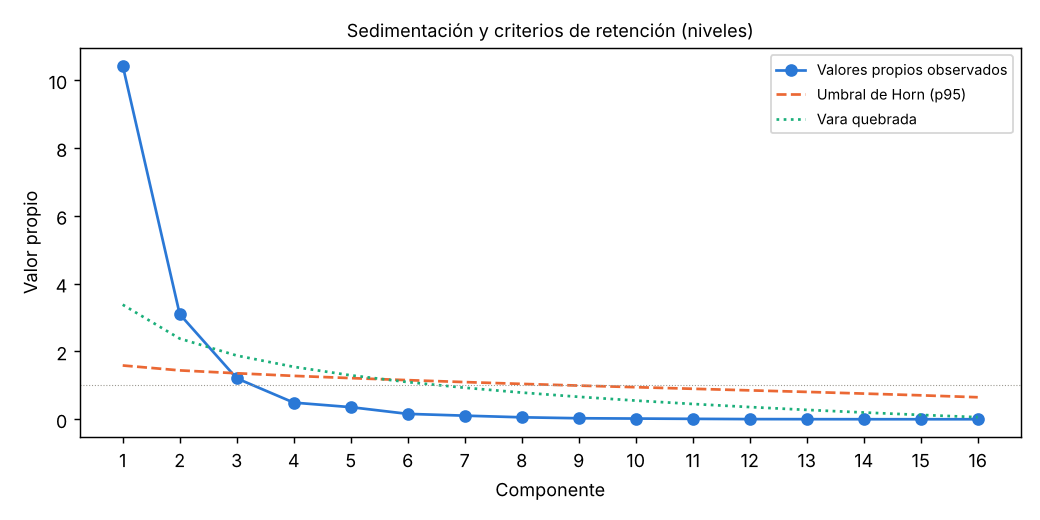
\includegraphics[width=0.75\textwidth]{final/05_pca_sedimentacion.png}
\caption{Valores propios del PCA global y umbrales de retención}
\label{fig:res-sedimentacion}
\par\smallskip
{\footnotesize Fuente: \texttt{reports/figures/final/05\_pca\_sedimentacion.png} (notebook 05).}
\end{figure}

\paragraph{Interpretación de los ejes.} Las cargas (\texttt{05\_pca\_cargas.csv}) permiten leer
los tres ejes retenidos:

\begin{itemize}[leftmargin=*]
  \item \textbf{Primer eje: profundización.} Cargan alto y con el mismo signo el crédito a
    empresas, de consumo e hipotecario, los agregados M1 y M3, el IPC, el PBI, la demanda interna y
    las reservas internacionales; también el tipo de cambio y, más débilmente, el índice bursátil.
    La tasa activa (TAMN) carga con signo opuesto. Es el eje del crecimiento conjunto de los
    agregados nominales y reales a lo largo de la muestra.
  \item \textbf{Segundo eje: tasas de interés de corto plazo.} Lo forman la tasa de referencia, la
    tasa interbancaria y la tasa pasiva (TIPMN), con cargas altas del mismo signo; la TAMN
    participa en menor grado.
  \item \textbf{Tercer eje: riesgo de mercado.} Opone el EMBIG, con carga positiva alta, al índice
    bursátil, con carga negativa; el tipo de cambio acompaña al EMBIG. Es el eje en que el aumento
    del riesgo soberano coincide con la caída de la bolsa.
\end{itemize}

\paragraph{Estabilidad de los ejes.} En el bootstrap por bloques con $\Lb=\largoBloqueNulo$, el
percentil 5 de la congruencia de Tucker (\cref{def:tucker}) entre cada eje original y su
emparejado en las réplicas es \congruenciaBootPCUnoNiveles{} para el primero,
\congruenciaBootPCDosNiveles{} para el segundo, \congruenciaBootPCTresNiveles{} para el tercero y
\congruenciaBootPCCuatroNiveles{} para el cuarto. Los tres primeros ejes son, por tanto,
descriptivamente estables; el cuarto no lo es, lo que respalda no interpretarlo. Con series no
estacionarias, este bootstrap mide estabilidad descriptiva y no incertidumbre muestral
(\cref{sec:met-pca}).

% -----------------------------------------------------------------------------
\section{Tendencia y nulo de tendencias}
\label{sec:res-tendencia}

\paragraph{El primer eje es una tendencia.} La correlación del primer componente con el tiempo es
\rTiempoPCUnoNiveles{}: el primer eje es, casi exactamente, una tendencia creciente. La regla de la
decisión D5 (\cref{def:regla-d5}) clasifica los cuatro primeros componentes como
\claseDCincoPCUnoNiveles{}, \claseDCincoPCDosNiveles{}, \claseDCincoPCTresNiveles{} y
\claseDCincoPCCuatroNiveles{}, respectivamente: sus residuos alrededor de una recta se comportan como
una tendencia estocástica. Entre las series, \nSeriesTS{} resulta estacionaria en tendencia (el
EMBIG), \nSeriesDS{} resultan integradas y \nSeriesIndeterminadas{} quedan indeterminadas (el
crédito de consumo, la TIPMN y el PBI). Como advierte \textcite{perron_1989}, una muestra con
quiebres, como la que contiene la crisis global y la pandemia, puede inclinar estas pruebas hacia
la raíz unitaria; la clasificación es un insumo del nulo, no una afirmación sobre el proceso
generador. La \cref{fig:res-residuos} muestra los residuos de cada componente alrededor de su
recta, con los episodios de referencia sombreados.

\begin{figure}[htbp]
\centering
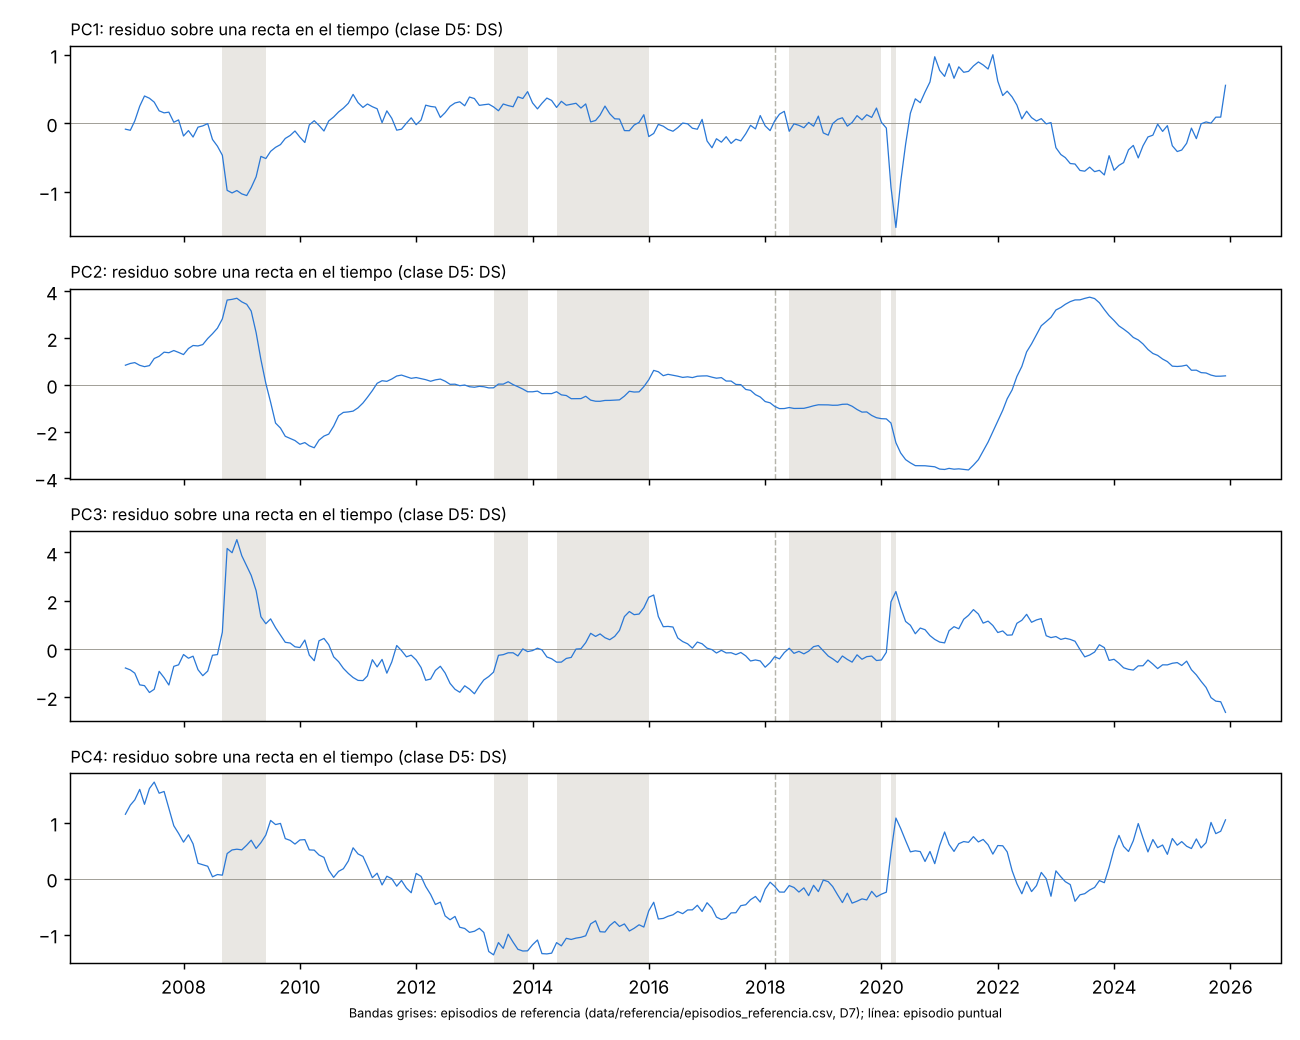
\includegraphics[width=0.85\textwidth]{final/05_pca_residuos_tendencia.png}
\caption{Residuos de los cuatro primeros componentes alrededor de una recta en el tiempo}
\label{fig:res-residuos}
\par\smallskip
{\footnotesize Fuente: \texttt{reports/figures/final/05\_pca\_residuos\_tendencia.png} (notebook
05). Bandas: episodios de referencia (\cref{tab:episodios}); línea discontinua: episodio puntual.}
\end{figure}

\paragraph{Nulo de tendencias mixto.} La pregunta es si la inercia de cada eje supera lo que
producirían series independientes, cada una con su propia tendencia y su propia dinámica
(\cref{def:nulo-mixto}; decisiones D8 y D19). Con el EMBIG y las series indeterminadas tratadas
como estacionarias en tendencia, la proporción de réplicas cuya inercia iguala o supera la
observada es \nuloMixtoTsPCUno{} para el primer eje, \nuloMixtoTsPCDos{} para el segundo y
\nuloMixtoTsPCTres{} para el tercero; tratadas como integradas, es \nuloMixtoDsPCUno{},
\nuloMixtoDsPCDos{} y \nuloMixtoDsPCTres{}. Las dos variantes coinciden en la lectura:

\begin{itemize}[leftmargin=*]
  \item la inercia del \textbf{primer eje no supera} lo esperable en series independientes con su
    propia tendencia: buena parte de su tamaño se debe a que las series crecen juntas en el tiempo,
    no a una relación común más allá de ese crecimiento;
  \item la del \textbf{segundo eje sí lo supera}: el comovimiento de las tasas de interés es real,
    no un efecto de las tendencias;
  \item la del tercer eje no lo supera con claridad.
\end{itemize}

Los nulos globales de la decisión D2 enmarcan este resultado. Con deriva en todas las series, la
proporción es \nuloConDerivaPCUno{} para el primer eje y \nuloConDerivaPCDos{} para el segundo; sin
deriva, \nuloSinDerivaPCUno{} y \nuloSinDerivaPCDos{}. La conclusión sobre el primer eje depende,
pues, de que las series tengan deriva, y el nulo mixto, que decide serie por serie con el
estadístico HAC (\cref{def:hac}), la resuelve a favor de la lectura con deriva.

\paragraph{Sin la tendencia lineal.} Como diagnóstico (decisión D5), al quitar a cada serie su
recta, el primer eje retiene \inerciaPCUnoSinTendencia\,\% de la inercia y la medida KMO baja a
\kmoSinTendencia{}; frente al nulo sin tendencia, la proporción para el primer eje es
\nuloSinTendenciaPCUno{}. La estructura común se debilita mucho cuando se quita la tendencia, lo
que confirma que esta domina la estructura de las series sin transformar.

\emph{Lectura.} En niveles, el primer eje mide sobre todo la profundización financiera y el
crecimiento nominal de la economía, no un ciclo. La estructura de interés para el ciclo financiero
está en los ejes siguientes, y sobre todo en el de tasas, que es el único que supera con claridad el
nulo de tendencias.

% -----------------------------------------------------------------------------
\section{Parte dinámica: EPCA, ancho de ventana y transiciones}
\label{sec:res-dinamica}

\subsection{Valores propios por ventana}
\label{sec:res-umbrales}

El algoritmo \texttt{aede} se ejecutó con los cuatro anchos de la grilla y los dos esquemas de
pesos. Con los anchos de 24, 36, 48 y 60 meses hay, respectivamente, \ventanasAedeVeinticuatro{},
\ventanasAedeTreintayseis{}, \ventanasAedeCuarentayocho{} y \ventanasAedeSesenta{} ventanas. La
\cref{tab:res-horn} compara el segundo y el tercer valor propio de cada ventana con el umbral de
Horn por ventana (\cref{def:umbral-ventana}; decisión D14).

\begin{table}[htbp]
\centering
\small
\caption{Ventanas en que el segundo y el tercer valor propio no superan el umbral de Horn}
\label{tab:res-horn}
\begin{tabular}{@{}>{\raggedright\arraybackslash}p{0.2\textwidth}C{0.16\textwidth}C{0.16\textwidth}C{0.16\textwidth}C{0.16\textwidth}@{}}
\toprule
 & \multicolumn{2}{c}{$\lambda_2(t)$ bajo el umbral} & \multicolumn{2}{c}{$\lambda_3(t)$ bajo el umbral} \\
\cmidrule(lr){2-3}\cmidrule(lr){4-5}
Ancho $\nw$ (ventanas) & Uniformes & Gaussianos & Uniformes & Gaussianos \\
\midrule
24 (\ventanasAedeVeinticuatro) & \bajoHornDosVeinticuatroU & \bajoHornDosVeinticuatroG & \bajoHornTresVeinticuatroU & \bajoHornTresVeinticuatroG \\
36 (\ventanasAedeTreintayseis) & \bajoHornDosTreintayseisU & \bajoHornDosTreintayseisG & \bajoHornTresTreintayseisU & \bajoHornTresTreintayseisG \\
48 (\ventanasAedeCuarentayocho) & \bajoHornDosCuarentayochoU & \bajoHornDosCuarentayochoG & \bajoHornTresCuarentayochoU & \bajoHornTresCuarentayochoG \\
60 (\ventanasAedeSesenta) & \bajoHornDosSesentaU & \bajoHornDosSesentaG & \bajoHornTresSesentaU & \bajoHornTresSesentaG \\
\bottomrule
\end{tabular}

\smallskip
\begin{minipage}{0.92\textwidth}\footnotesize
Fuente: \texttt{data/results/final/06c\_aede\_valores\_propios\_resumen.csv} (notebook 06c). Con
pesos gaussianos, el umbral usa el tamaño efectivo de la \cref{tab:kish}.
\end{minipage}
\end{table}

Tres resultados se desprenden de la tabla y del archivo de origen. Primero, el primer valor propio
supera los umbrales de Kaiser y de Horn en todas las ventanas, con todos los anchos y pesos: la
coherencia unidimensional del sistema nunca desaparece. Segundo, el segundo valor propio queda bajo
el umbral de Horn en buena parte de las ventanas cortas y en pocas de las largas: el eje de tasas
solo se distingue con claridad del ruido a escalas de cuatro o cinco años. Tercero, el tercer valor
propio queda bajo el umbral en la mayoría de las ventanas con todos los anchos: el eje de riesgo de
mercado, que el PCA global retiene por la decisión D9, no se sostiene ventana por ventana. Con el
ancho de 24 meses hay, además, \ventanasSerieConstanteVeinticuatro{} ventanas en que alguna serie es
constante y quedan fuera de la \cref{def:epca}; se registran también cruces entre el segundo y el
tercer valor propio con todos los anchos (\cref{obs:aede}(b)).

La \cref{fig:res-varianza} muestra, para el ancho de 60 meses de la regla del 06, la evolución de
la varianza explicada por el segundo y el tercer eje, y la \cref{fig:res-cargas}, la de las cargas
del segundo eje. La composición del segundo eje cambia: en unos tramos lo dominan las tasas de
interés y en otros el EMBIG o el índice bursátil.

\begin{figure}[htbp]
\centering
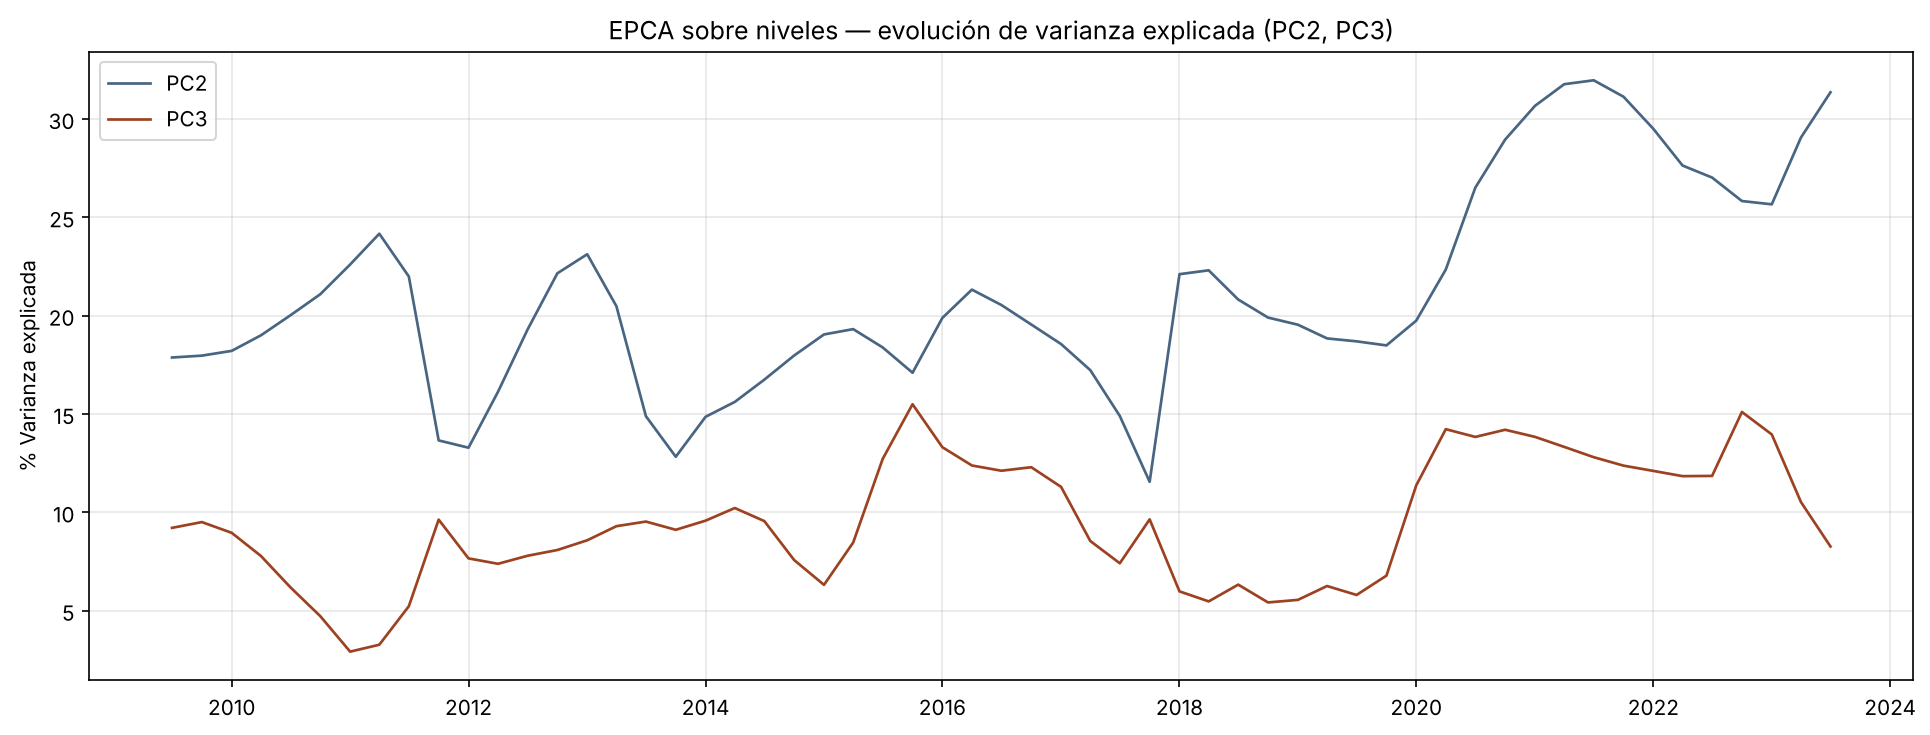
\includegraphics[width=0.95\textwidth]{final/06_epca_varianza_evolutiva_niveles.png}
\caption{Varianza explicada por el segundo y el tercer eje en ventanas de 60 meses}
\label{fig:res-varianza}
\par\smallskip
{\footnotesize Fuente: \texttt{reports/figures/final/06\_epca\_varianza\_evolutiva\_niveles.png}
(notebook 06; ventanas con paso de \pasoReglaSeis{} meses, fechadas en su centro).}
\end{figure}

\begin{figure}[htbp]
\centering
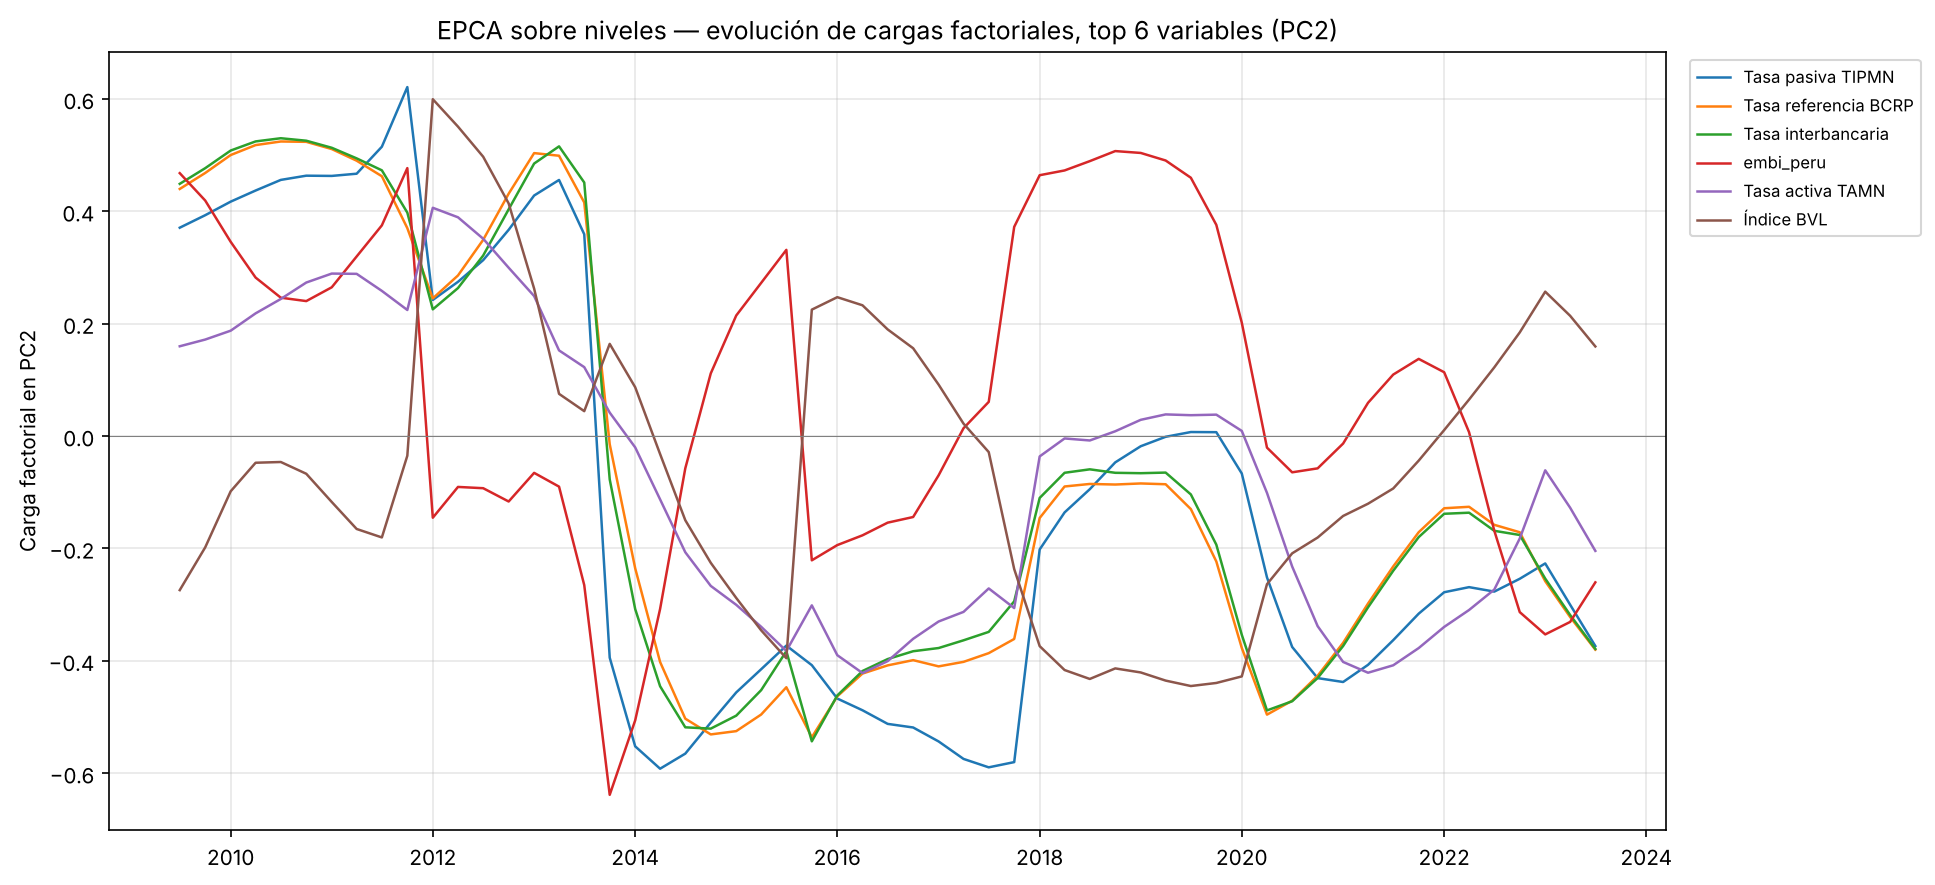
\includegraphics[width=0.95\textwidth]{final/06_epca_cargas_evolutivas_niveles.png}
\caption{Cargas del segundo eje en ventanas de 60 meses (series con mayor carga)}
\label{fig:res-cargas}
\par\smallskip
{\footnotesize Fuente: \texttt{reports/figures/final/06\_epca\_cargas\_evolutivas\_niveles.png}
(notebook 06).}
\end{figure}

\subsection{Número de segmentos de \texttt{aede}}
\label{sec:res-aede}

Con $K_{\max}=10$, el codo por caída máxima de la partición de $\lambda_1$
(\cref{def:criterios-k}(a)) elige dos segmentos, es decir, un único corte, con todos los anchos y
pesos salvo uno: con 24 meses y pesos uniformes elige \kCodoVeinticuatroU{} segmentos. Con los
anchos de 36, 48 y 60 meses, el único corte cae cerca del inicio de la pandemia: con pesos
uniformes y gaussianos, en \corteCodoTreintayseisU{} y \corteCodoTreintayseisG{} (36 meses),
\corteCodoCuarentayochoU{} y \corteCodoCuarentayochoG{} (48 meses) y \corteCodoSesentaU{} y
\corteCodoSesentaG{} (60 meses). Con 24 meses y pesos gaussianos, el corte cae en
\corteCodoVeinticuatroG{}. Los cortes se fechan en el centro de la primera ventana del segmento
siguiente (\cref{alg:aede}).

Frente al nulo de estructura constante (\cref{def:nulo-estructura}), el número de segmentos que
elige el codo está dentro del rango central de las réplicas con todos los anchos
(\texttt{07b\_nulo\_estructura\_kstar\_posicion.csv}): una estructura constante produciría, con
estos datos, un número de cortes similar. Las dos variantes del índice de Caliński y Harabasz
eligen el máximo de la grilla en casi todas las combinaciones, y lo mismo ocurre en casi todas las
réplicas del nulo, como anticipan la \cref{prop:ch} y la \cref{obs:ch}. Por la decisión D11, el
índice no se usa como selector: no muestra un óptimo interior fuera del rango del nulo.

\subsection{Criterio de ancho de ventana (OE4)}
\label{sec:res-oe4}

La \cref{tab:res-oe4} presenta el criterio de la \cref{def:oe4} para cada ancho y esquema de
pesos, con el RV de cargas de tres ejes como objeto principal (decisión D17.2) y el nulo de
estructura constante con $\Lb=\largoBloqueNulo$ y $B=\replicasNuloEstructura$ réplicas.

\begin{table}[htbp]
\centering
\small
\caption{Criterio de OE4: proporción de pares de ventanas adyacentes bajo el umbral del nulo y su
p-valor}
\label{tab:res-oe4}
\begin{tabular}{@{}lC{0.18\textwidth}C{0.18\textwidth}C{0.18\textwidth}C{0.18\textwidth}@{}}
\toprule
 & \multicolumn{2}{c}{Pesos uniformes} & \multicolumn{2}{c}{Pesos gaussianos} \\
\cmidrule(lr){2-3}\cmidrule(lr){4-5}
Ancho $\nw$ & $\varpi_0$ & $\pval$ & $\varpi_0$ & $\pval$ \\
\midrule
24 & \propOEcuatroVeinticuatroU & \pOEcuatroVeinticuatroU & \propOEcuatroVeinticuatroG & \pOEcuatroVeinticuatroG \\
36 & \propOEcuatroTreintayseisU & \pOEcuatroTreintayseisU & \propOEcuatroTreintayseisG & \pOEcuatroTreintayseisG \\
48 & \propOEcuatroCuarentayochoU & \pOEcuatroCuarentayochoU & \propOEcuatroCuarentayochoG & \pOEcuatroCuarentayochoG \\
60 & \propOEcuatroSesentaU & \pOEcuatroSesentaU & \propOEcuatroSesentaG & \pOEcuatroSesentaG \\
\bottomrule
\end{tabular}

\smallskip
\begin{minipage}{0.92\textwidth}\footnotesize
Fuente: \texttt{data/results/final/07b\_nulo\_estructura\_oe4.csv} (notebook 07b), filas
principales. $\varpi_0$: proporción observada de pares bajo el percentil 5 por posición del nulo;
$\pval$: proporción de réplicas con una proporción igual o mayor (\cref{def:oe4}).
\end{minipage}
\end{table}

En ningún ancho ni esquema de pesos el p-valor es menor que el nivel de 5\,\%: la proporción de
pares de ventanas adyacentes con un RV inusualmente bajo no es mayor que la que produce una
estructura constante. Las sensibilidades (el coeficiente entre matrices de correlación completas y
las longitudes de bloque de \largoBloqueNuloCorto{} y \largoBloqueNuloLargo{} meses) conducen a la
misma lectura (\texttt{07b\_nulo\_estructura\_oe4.csv}).

El resultado no significa que la estructura sea constante. Los RV observados entre ventanas
adyacentes son bajos, es decir, la configuración de las cargas cambia mucho de un bloque de
$\nw$ meses al siguiente; pero las réplicas del nulo, que acumulan incrementos remuestreados,
producen cambios igual de grandes. Con series integradas, la correlación de una ventana es muy
variable aunque la estructura de los incrementos sea la misma, y el nulo lo reproduce
(\cref{obs:nulo-estructura}(b)). El criterio de OE4 queda así formalizado y calculado, pero, con
las series sin transformar, no discrimina ningún ancho: los cuatro son compatibles con una
estructura constante. Esa es una información sustantiva para la Parte~C de D2.

\subsection{Transiciones candidatas y lectura de octubre de 2017}
\label{sec:res-transiciones}

Las transiciones candidatas son las de la regla del 06 con cada ancho y los cortes del codo de
\texttt{aede}; en total, \nTransicionesCandidatas{} candidatas en el objeto principal. La
\cref{fig:res-transiciones} muestra la regla del 06 con el ancho de 60 meses: la estabilidad del
segundo eje cae bajo el umbral en varias ocasiones. Casi todas las candidatas, con todos los anchos,
coinciden con un borde de ventana, es decir, con la entrada o la salida de un episodio de la
ventana (\cref{def:borde}), o quedan dentro del nulo (\cref{def:fuera-nulo}). Solo
\nTransicionesCuentan{} candidata no es un borde y está fuera del nulo, en
\transicionCuentaFecha{}, con la regla del 06 y el ancho de 36 meses
(\texttt{07b\_transiciones\_d10.csv}).

\begin{figure}[htbp]
\centering
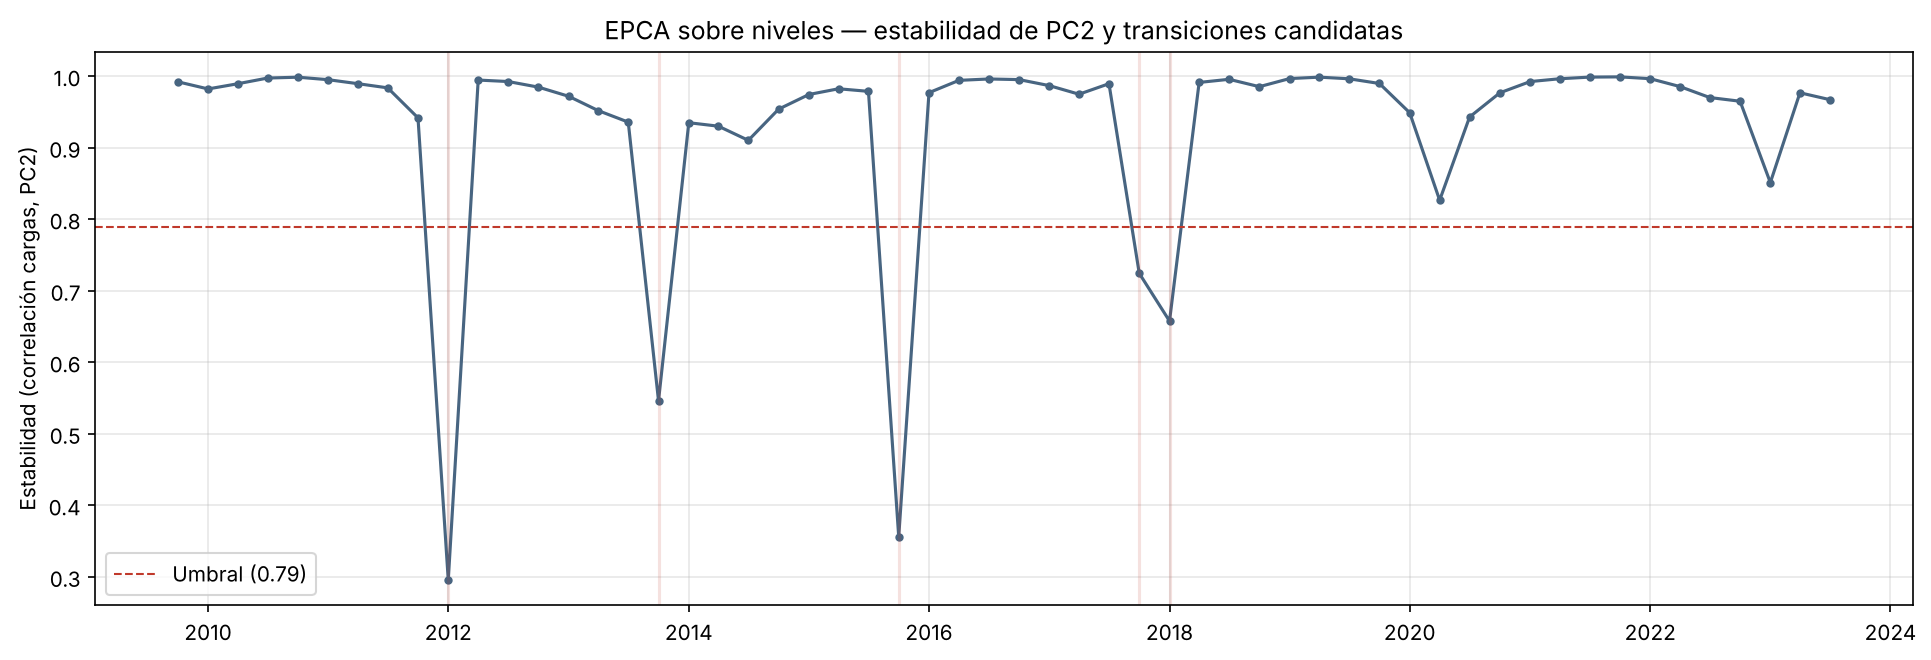
\includegraphics[width=0.95\textwidth]{final/06_epca_transiciones_niveles.png}
\caption{Regla del 06: estabilidad del segundo eje entre ventanas sucesivas de 60 meses}
\label{fig:res-transiciones}
\par\smallskip
{\footnotesize Fuente: \texttt{reports/figures/final/06\_epca\_transiciones\_niveles.png} (notebook
06). Línea discontinua: umbral $\bar\rho-s_\rho$ de la \cref{def:regla06}; líneas verticales:
transiciones candidatas.}
\end{figure}

La transición de octubre de 2017, que la decisión D13 menciona por su nombre, aparece solo con la
regla del 06 y el ancho de 60 meses; en ese ancho coincide con un borde de ventana (la entrada de la
pandemia en la ventana) y no está fuera del nulo. No cumple, pues, ninguna de las dos condiciones de
la \cref{def:confirmada}, y se informa como \textbf{transición no confirmada}
(\texttt{07b\_clasificacion\_2017\_10.csv}), tanto con el objeto principal como con la sensibilidad.

% -----------------------------------------------------------------------------
\section{Clasificación Factorial Jerárquica}
\label{sec:res-hfc}

La HFC (\cref{def:hfc}) cortada en \clasesHfcMenor{} clases separa \clasesHfcMenor{} bloques
(\cref{tab:res-hfc}). La composición se lee de \texttt{07c\_hfc\_clases3.csv}; el representante es
la serie de la clase más correlacionada, en valor absoluto, con el factor (definición operativa del
código, pendiente de consulta con el asesor; \cref{sec:pend-representante}).

\begin{table}[htbp]
\centering
\small
\caption{Partición de la HFC en \clasesHfcMenor{} clases}
\label{tab:res-hfc}
\begin{tabular}{@{}l>{\raggedright\arraybackslash}p{0.5\textwidth}>{\raggedright\arraybackslash}p{0.25\textwidth}@{}}
\toprule
Clase & Series & Representante \\
\midrule
C1 & Crédito a empresas, de consumo e hipotecario; M1 y M3; IPC; tipo de cambio; PBI; demanda
  interna; reservas internacionales; TAMN (con signo opuesto) & Crédito hipotecario \\
C2 & Tasa de referencia, tasa interbancaria y TIPMN & Tasa interbancaria \\
C3 & EMBIG e índice bursátil (con signos opuestos) & EMBIG \\
\bottomrule
\end{tabular}

\smallskip
\begin{minipage}{0.92\textwidth}\footnotesize
Fuente: \texttt{data/results/final/07c\_hfc\_clases3.csv} (notebook 07c). Las clases se identifican
por su composición, no por el número del nodo.
\end{minipage}
\end{table}

Las \clasesHfcMenor{} clases reproducen los tres ejes retenidos del PCA: C1 es el bloque de la profundización (primer
eje), C2 el de las tasas de corto plazo (segundo eje) y C3 el del riesgo de mercado (tercer eje). La
partición en \clasesHfcMayor{} clases solo separa el EMBIG y el índice bursátil en clases propias.

\paragraph{Estabilidad.} En \replicasHfc{} réplicas del bootstrap por bloques, el índice de Rand
ajustado entre la partición en \clasesHfcMenor{} clases de cada réplica y la original tiene mediana
\ariTresMediana{} y media \ariTresMedia{}: la partición en \clasesHfcMenor{} clases se reproduce casi siempre.
La partición en \clasesHfcMayor{} clases es menos estable (media \ariCuatroMedia{}), porque la separación
entre el EMBIG y el índice bursátil depende de la réplica. La correlación cofenética entre la
jerarquía de cada réplica y la original tiene mediana \cofeneticaMediana{}.

\paragraph{Relación entre las clases.} La correlación entre los factores de C1 y C3 es
\rFactoresUnoTres{}, con un intervalo bootstrap de \rFactoresUnoTresPcinco{} a
\rFactoresUnoTresPnoventaycinco{} que no contiene el cero; las demás correlaciones entre factores
tienen intervalos que sí lo contienen (\texttt{07c\_hfc\_correlaciones3.csv}). Al quitar la
tendencia lineal de cada serie, la relación que se destaca es otra: la de los factores de C1 y C2,
con correlación \rFactoresUnoDosSinTendencia{} e intervalo de
\rFactoresUnoDosSinTendenciaPcinco{} a \rFactoresUnoDosSinTendenciaPnoventaycinco{}. Las relaciones
entre bloques dependen, pues, de que se incluya o no la tendencia, y deben leerse con la misma
cautela que el primer eje del PCA.

\paragraph{Comparación con el antecedente.} \textcite{camiz_cerda_atoche_2026} encuentran tres
grupos: salud económica y financiera, tasas de interés y riesgo del mercado financiero
(\cref{sec:antecedentes}). La correspondencia por bloque (HT2) es la siguiente. El bloque de tasas
coincide en esencia, salvo que aquí la tasa activa queda en C1 y no con las demás tasas. El bloque
de riesgo coincide en el EMBIG y el índice bursátil, pero las reservas internacionales quedan aquí
en C1, y el coeficiente de dolarización no forma parte de las \nSeries{} series. C1 corresponde al
bloque de salud económica y financiera, ampliado con el tipo de cambio y la actividad, que el
antecedente trata de otra manera: el tipo de cambio, en particular, queda fuera de su análisis
principal. Como los conjuntos de series no son idénticos, la comparación es por bloque y no serie a
serie.

\pendiente{figura del dendrograma de la HFC con la partición en \clasesHfcMenor{} clases, generada desde el
notebook 07c o el Rmd final y guardada en \texttt{reports/figures/final/}}

% -----------------------------------------------------------------------------
\section{Datación de regímenes}
\label{sec:res-datacion}

La datación PCA-MM\ventanaMediaMovil{} (\cref{def:datacion}) particiona la trayectoria de los tres
primeros \emph{scores} suavizados, con longitud mínima de 12 meses. Con $K_{\max}=10$ (decisión
D17.1), la regla K (\cref{def:criterios-k}(b)) elige \nRegimenesPrincipal{} regímenes; el primer
paso de la regla no elige ningún número dentro de la grilla y la elección la hace el segundo paso,
el codo. Los cortes, en el primer mes de cada régimen nuevo, son \corteDatacionUno{},
\corteDatacionDos{}, \corteDatacionTres{}, \corteDatacionCuatro{} y \corteDatacionCinco{}. La
\cref{tab:res-regimenes} los resume con la estabilidad de cada corte en las réplicas del bootstrap
y con la etiqueta de fase de la regla del notebook 09.

\begin{table}[htbp]
\centering
\small
\caption{Regímenes de la datación principal}
\label{tab:res-regimenes}
\begin{tabular}{@{}cC{0.19\textwidth}C{0.19\textwidth}lC{0.2\textwidth}@{}}
\toprule
Régimen & Inicio & Fin & Fase (preliminar) & Estabilidad del corte inicial \\
\midrule
1 & \regimenUnoInicio & \regimenUnoFin & Transición & --- \\
2 & \regimenDosInicio & \regimenDosFin & Transición & \estabilidadCorteUno \\
3 & \regimenTresInicio & \regimenTresFin & Contracción & \estabilidadCorteDos \\
4 & \regimenCuatroInicio & \regimenCuatroFin & Transición & \estabilidadCorteTres \\
5 & \regimenCincoInicio & \regimenCincoFin & Expansión & \estabilidadCorteCuatro \\
6 & \regimenSeisInicio & \regimenSeisFin & Expansión & \estabilidadCorteCinco \\
\bottomrule
\end{tabular}

\smallskip
\begin{minipage}{0.95\textwidth}\footnotesize
Fuente: \texttt{data/results/final/09a\_regimenes\_pca.csv} y \texttt{09a\_estabilidad\_cortes.csv}
(notebook 09a). Estabilidad: proporción de las \replicasDatacion{} réplicas del bootstrap que
reproducen el corte con la tolerancia de 3 meses. La etiqueta de fase es la de la regla del
notebook 09, propuesta preliminar pendiente de discusión con el asesor (\cref{def:fase}).
\end{minipage}
\end{table}

Cuatro rasgos acotan la lectura de la tabla:

\begin{enumerate}[leftmargin=*]
  \item \textbf{El número de regímenes depende de la regla.} Con $K_{\max}=15$ y $K_{\max}=20$, el
    primer paso de la regla K sí elige, y da \nRegimenesQuince{} y \nRegimenesVeinte{} regímenes.
    La especificación principal es la de $K_{\max}=10$ por la decisión D17.1, fijada antes de
    calcular; pero el resultado muestra que el número de regímenes no es una propiedad robusta de
    los datos, sino de la regla que lo fija.
  \item \textbf{No todos los cortes son estables.} La mayoría de los cortes se reproduce en una
    proporción alta de las réplicas, pero el corte de \corteDatacionTres{} se reproduce en menos de
    la mitad.
  \item \textbf{La dimensión importa.} Con $d=2$ y $d=4$ (decisión D9), la regla K elige
    \nRegimenesDimDos{} y \nRegimenesDimCuatro{} regímenes, con cortes que solo en parte coinciden
    con los de $d=3$ (\texttt{09a\_datacion\_dimension.csv}).
  \item \textbf{El primer régimen tiene la longitud mínima} de 12 meses: está condicionado por la
    restricción y no solo por los datos (\cref{cor:fisher-factible}).
\end{enumerate}

\emph{Lectura.} La datación distingue un tramo inicial alrededor de la crisis financiera global, un
largo tramo intermedio y un tramo posterior a la pandemia; las fases preliminares asignan
contracción al período posterior a la crisis y expansión al período pospandemia. Como la
trayectoria particionada incluye el primer eje, que es sobre todo tendencia
(\cref{sec:res-tendencia}), parte de lo que separan los cortes es el avance de esa tendencia, y no
solo cambios de estructura. La distinción entre ambos componentes es una de las preguntas de la
Parte~C.

\pendiente{figura de la trayectoria PCA-MM\ventanaMediaMovil{} con los cortes de la datación
principal y los episodios de referencia, generada desde el notebook 09a o el Rmd final y guardada
en \texttt{reports/figures/final/}}

% -----------------------------------------------------------------------------
\section{Contraste con los episodios de referencia}
\label{sec:res-validacion}

La hipótesis HT3 se evalúa con los episodios de la \cref{tab:episodios}, fechados por eventos
externos al análisis (decisiones D7 y D18), con la tolerancia principal de 3 meses y la de
sensibilidad de 6 (\cref{def:tolerancia}). Con pocos episodios, algunos puntuales, la
correspondencia es descriptiva y no tiene poder estadístico.

\paragraph{Datación principal.} El archivo de regímenes registra qué episodios caen dentro de cada
régimen (\texttt{09a\_regimenes\_pca.csv}). Los dos primeros regímenes contienen la crisis
financiera global: el primer corte cae dentro de ese episodio. El tercer régimen contiene el
\emph{taper tantrum}. El cuarto régimen es largo y contiene varios episodios: el colapso de las
materias primas, la renuncia de Kuczynski, la guerra comercial y la pandemia; la datación no los
separa. El quinto régimen empieza poco después del fin del episodio de la pandemia, y el último
corte no corresponde a ningún episodio de la lista, que no incluye eventos posteriores a la
pandemia; ese corte queda sin contraste externo.
\pendiente{tabla de compatibilidad de cada corte con cada episodio, con $h=3$ y $h=6$
(\cref{def:tolerancia}), a generar por el desarrollador desde \texttt{09a\_regimenes\_pca.csv} y
\texttt{data/referencia/episodios\_referencia.csv}; sin ella, la correspondencia anterior se
describe por contención y no por distancia}

\paragraph{\texttt{aede}.} Los cortes únicos del codo con los anchos de 36 a 60 meses se agrupan
alrededor de la pandemia (\cref{sec:res-aede}). Es el choque más abrupto de la muestra, como se aprecia en la \cref{fig:res-residuos}, y el único
episodio que todos esos anchos registran. Pero esos cortes están dentro del rango del nulo de estructura
constante, y algunos coinciden con un borde de ventana, de modo que no cuentan como transiciones
confirmadas.

\paragraph{Detección fuera de muestra.} La detección de episodios con la razón de error
\emph{walk-forward} del PCA solo es informativa con las series transformadas, y se presenta en el
anexo de robustez (\cref{sec:ap-deteccion}).

\emph{Lectura.} Los episodios más intensos, la crisis global y la pandemia, se reflejan en la
datación y, la pandemia, también en el EPCA. Los episodios de menor intensidad o más cercanos entre
sí no se separan. La correspondencia con HT3 es, por tanto, parcial, y con la salvedad, que la
propia hipótesis anticipa en su contra, de que el número de cortes depende de la regla que lo fija.

% -----------------------------------------------------------------------------
\section{Aprendizaje profundo: estado del complemento}
\label{sec:res-dl}

Los autoencoders y las redes LSTM se entrenaron en iteraciones anteriores con 17 series, con la
liquidez M2 incluida, en las dos vías, siguiendo el diseño de la \cref{sec:dl}: anclaje en el
autoencoder lineal, validación por bloques temporales, estabilidad entre réplicas medida con el
coeficiente RV y detección \emph{walk-forward}. Por la decisión D17.4, esos resultados se conservan
como antecedente (commit \texttt{2be3665}) y no se usan en esta tesis, y los modelos se volverán a
entrenar con las \nSeries{} series vigentes en la iteración 4, cuando el entorno de cómputo disponga
de la biblioteca \texttt{torch} (\cref{sec:pend-dl}). La hipótesis HT4 y los objetivos
\labelcref{oe:dl,oe:incertidumbre} quedan, por ahora, sin evaluar.

% -----------------------------------------------------------------------------
\section{Discusión}
\label{sec:res-discusion}

Esta sección contrasta los resultados con las hipótesis de trabajo de la \cref{sec:hipotesis}. Cada
hipótesis declaró de antemano qué resultado contaría en su contra; la discusión usa esos criterios.

\paragraph{HT1 (no estacionariedad estructural): no sostenida por el criterio formal en niveles.}
Descriptivamente, la estructura cambia: el segundo y el tercer eje cambian de composición y de
peso entre ventanas (\cref{fig:res-varianza,fig:res-cargas}), y el RV entre ventanas adyacentes es
bajo. Pero el resultado que HT1 declaró en su contra se cumple: con las series sin transformar, las
ventanas sucesivas no son menos parecidas de lo que cabría esperar bajo una estructura constante,
con ningún ancho (\cref{tab:res-oe4}), y el número de cortes de \texttt{aede} es típico del nulo.
La explicación más probable es de potencia: con series integradas, el nulo de estructura constante
genera tanta variabilidad entre ventanas como los datos (\cref{obs:nulo-estructura}). Si esto es
así, la pregunta de HT1 debería contrastarse en una vía en que la variabilidad muestral de la
correlación sea menor, como la de las series transformadas; esa es una propuesta para la Parte~C, no
una conclusión.

\paragraph{HT2 (organización en grupos): sostenida en lo esencial.} Las series se organizan en \clasesHfcMenor{}
bloques estables bajo remuestreo (profundización, tasas y riesgo de mercado), que coinciden con los
tres ejes del PCA y se corresponden, por bloque, con los de \textcite{camiz_cerda_atoche_2026}. Las
diferencias (la tasa activa, el tipo de cambio y las reservas) son de asignación de series
individuales y se explican en parte por la diferencia de los conjuntos de datos. La partición en
\clasesHfcMayor{} clases es menos estable, de modo que el nivel de corte de \clasesHfcMenor{} clases es el que se sostiene.

\paragraph{HT3 (correspondencia con episodios): parcial.} Los episodios intensos se reflejan en la
datación, pero el número de regímenes depende de la regla que lo fija, uno de los cortes es poco
estable y un régimen largo agrupa varios episodios. Además, el primer eje, que pesa en la
trayectoria particionada, es sobre todo tendencia. HT3 queda parcialmente sostenida, con una
evidencia descriptiva que la tabla de compatibilidad pendiente permitirá precisar.

\paragraph{HT4 (complementariedad del aprendizaje profundo): sin evaluar.} Ver la
\cref{sec:res-dl}.

\paragraph{Qué sostienen los resultados, en conjunto.} Con las series sin transformar, la
estructura de los datos está dominada por una tendencia común de profundización; sobre ella, hay un
comovimiento de las tasas de interés que supera el nulo de tendencias y \clasesHfcMenor{} bloques de series
estables. Lo que los resultados en niveles \emph{no} sostienen todavía es que los cambios de
estructura en el tiempo sean distinguibles de los que produce una estructura constante. La
diferencia entre lo que mide cada vía (estructura y regímenes en niveles, detección en la vía
transformada) es exactamente la propuesta de la Parte~C de D2, que se discutirá con el asesor
antes de consolidar ninguna conclusión.
